\chapter{Specyfikacja techniczna}

\section{Architektura}

System został podzielony na moduły. Poszczególne moduły odpowiadają obiektom z domeny projektu i realizują następujące zadania:\\

\textbf{UAV\_physic\_engine} -- moduł odpowiedzialny symulację dynamiki statku powietrznego, uwzględniając wszystkie jego właściwości mechaniczne i wpływ otoczenia. Oblicza stan pojedynczego BSP w czasie rzeczywistym. \\

\textbf{UAV\_controller} -- moduł reprezentujący system sterowania statkiem powietrznym. Interpretuje stan statków powietrznych i buduje symulacje otoczenie. Symuluje działanie czujników pomiarowych, systemu filtracji, algorytmów nawigacji pokładowej oraz systemów sterowania i stabilizacji. Bezpośrednio wpływa na zachowanie symulacji dynamiki.\\

\textbf{UAV\_drop\_physic} -- moduł odpowiedzialny za obliczenie dynamiki pocisków. Oblicza stan wszystkich pocisków aktywnych w symulacji.\\

\textbf{UAV\_aggregator} -- moduł agregujący moduły symulacyjne z wizualizacją. Zarządza pracą pozostałych modeli i wprowadza niektóre zagadnienia otoczenia takie jak atmosferę, połączenia miedzy BSP, a ładunkami oraz kolizje.\\

\textbf{UAV\_server} -- definicja wirtualnego kontenera, odpowiedzialna zabudowanie wszystkich modułów składających się na serwer, tj. wszystkie z wyłączeniem wizualizacji. Ze zbudowanych modułów budowany jest obraz kontenera. Umożliwia to uruchomienie serwera na dowolnej maszynie wspierającej daną konteneryzację.\\

\textbf{UAV\_visualization} -- moduł odpowiedzialny za wyświetlenie  interfejsu użytkownika oraz obecnego stanu symulacji. Przekazuje dane wejściowe z kontrolera do systemu. Stanowi interfejs komunikacji użytkownika z systemem. \\

\textbf{UAV\_map\_generator} -- skrypt automatyzujący proces generowania mapy, w oparciu o dane geograficzne. \\

\section{Opis działania systemu}

W centralnym punkcie aplikacji znajduje się moduł agregatora. Stanowi on główną część serwera, jest aplikacją konsolową i nie posiada interfejsu graficznego. Jest zawsze uruchamiany jako pierwszy. Po rozpoczęciu pracy agregatora uruchamiany jest moduł "drop physic" jako podproces, a agregator nawiązuje z nim połączenie. Oba moduły pozostają w stanie bezczynności do momentu podłączenia się pierwszego użytkownika. Nowy użytkownik dodawany jest przez uruchomienie wizualizacji. Po uruchomieniu wizualizacji, komunikuje się ona z serwerem i prosi o~utworzenie nowego statku powietrznego. W odpowiedzi na to żądanie, agregator uruchamia jako swoje podprocesy "physic engine" i "controller".Następnie para procesów synchronizuje się ze sobą i rozpoczyna symulację. Każdemu symulowanemu statkowi powietrznemu odpowiada para procesów "physic engine" i "controller". Ponadto każdy statek jest kontrolowany z poziomu konkretnej wizualizacji.\\

W trakcie pracy systemu agregator pełni rolę pośrednika w komunikacji między wizualizacją a procesami silnika fizycznego i regulatora. Przesyła instrukcje sterujące z wizualizacji do odpowiedniej symulacji fizycznej, agreguje stany ze wszystkich aktywnych symulacji i przesyła je z powrotem do wizualizacji. Ponadto zarządza procesami strzału, upuszczania ładunku i kolizji.\\

Po odłączeniu się wizualizacji od serwera, procesy związane z danym statkiem są zamykane.


\section{Opis komponentów}

Kod poszczególnych modułów systemu został w całości opisany z wykorzystaniem narzędzi do dokumentowania kodu: Doxygen, JavaDoc i Rust Doc. Dla poszczególnych modułów wygenerowane zostały opisy klas oraz funkcji i załączone do pracy jako dokumenty PDF lub strony HTML.

\newpage

\section{Komunikacja}

Moduły komunikują się między sobą poprzez kolejki ZeroMQ\cite{zmqguide}. ZeroMQ to uniwersalna implementacja różnych wzorów komunikacji niezależna od języka i warstwy transportowej. Istnieją oficjalne biblioteki ZeroMQ przeznaczone do wykorzystania w projektach w językach  C++, Rust, Java, Python i wielu innych. Jako warstwa transportowa wykorzystane mogą być mechanizmy komunikacji wewnątrzprocesowej, międzyprocesowej i protokół TCP/IP oraz dowolne ich kombinację. Wzorami dostępnymi w kolejkach ZeroMQ, które zostaną wykorzystane w projekcie są:

\begin{itemize}
\item PUB--SUB -- jednokierunkowa komunikacja publikujący --  subskrybujący. Jest to połączenie jeden do wielu.  Wielu subskrybujących ma możliwość podłączenia się do jednego publikującego i zasubskrybowania określonych wiadomości (zdefiniowanych przez prefix). Publikujący rozsyła wiadomości do wszystkich podłączonych subskrybentów, którzy subskrybują dany typ wiadomości.

\item PAIR--PAIR -- uniwersalne połączenie jeden do jeden. Tworzy połączenie dwóch socketów, umożliwiające dwukierunkową komunikacje. Stanowi bezpośredni odpowiednich Unixowych pipe'ów lub surowego protokołu TCP.

\item REQ--REP -- model komunikacji klient serwer w której serwer (REP -- replyer) odpowiada na zapytania klienta (REQ -- requester). W modelu wielu klientów może odpytywać serwer, a ich żądania są kolejno obsługiwane i wysyłana jest na nie odpowiedź.
\end{itemize}

Oprócz wyżej przedstawionych istnieje również wiele wariacji modeli komunikacji pozwalające m. in. na rozdzielanie pracy na wiele serwerów (load balance) lub przekierowywanie wiadomości ze zmianą warstwy transportowej lub podsłuchem (proxy).\\

Rysunek (\ref{comm}) prezentuje poszczególne moduły oraz kanały komunikacji. Na niebiesko zaznaczone zostały kolejki TCP/IP, a na czerwono kolejki wykorzystujące mechanizmy IPC. Dla zwiększenia czytelności, kolejki w warstwie miedzy procesowej nie zostały zaznaczone na rysunku.

\newpage
 \begin{figure}[!h]
  \centering
  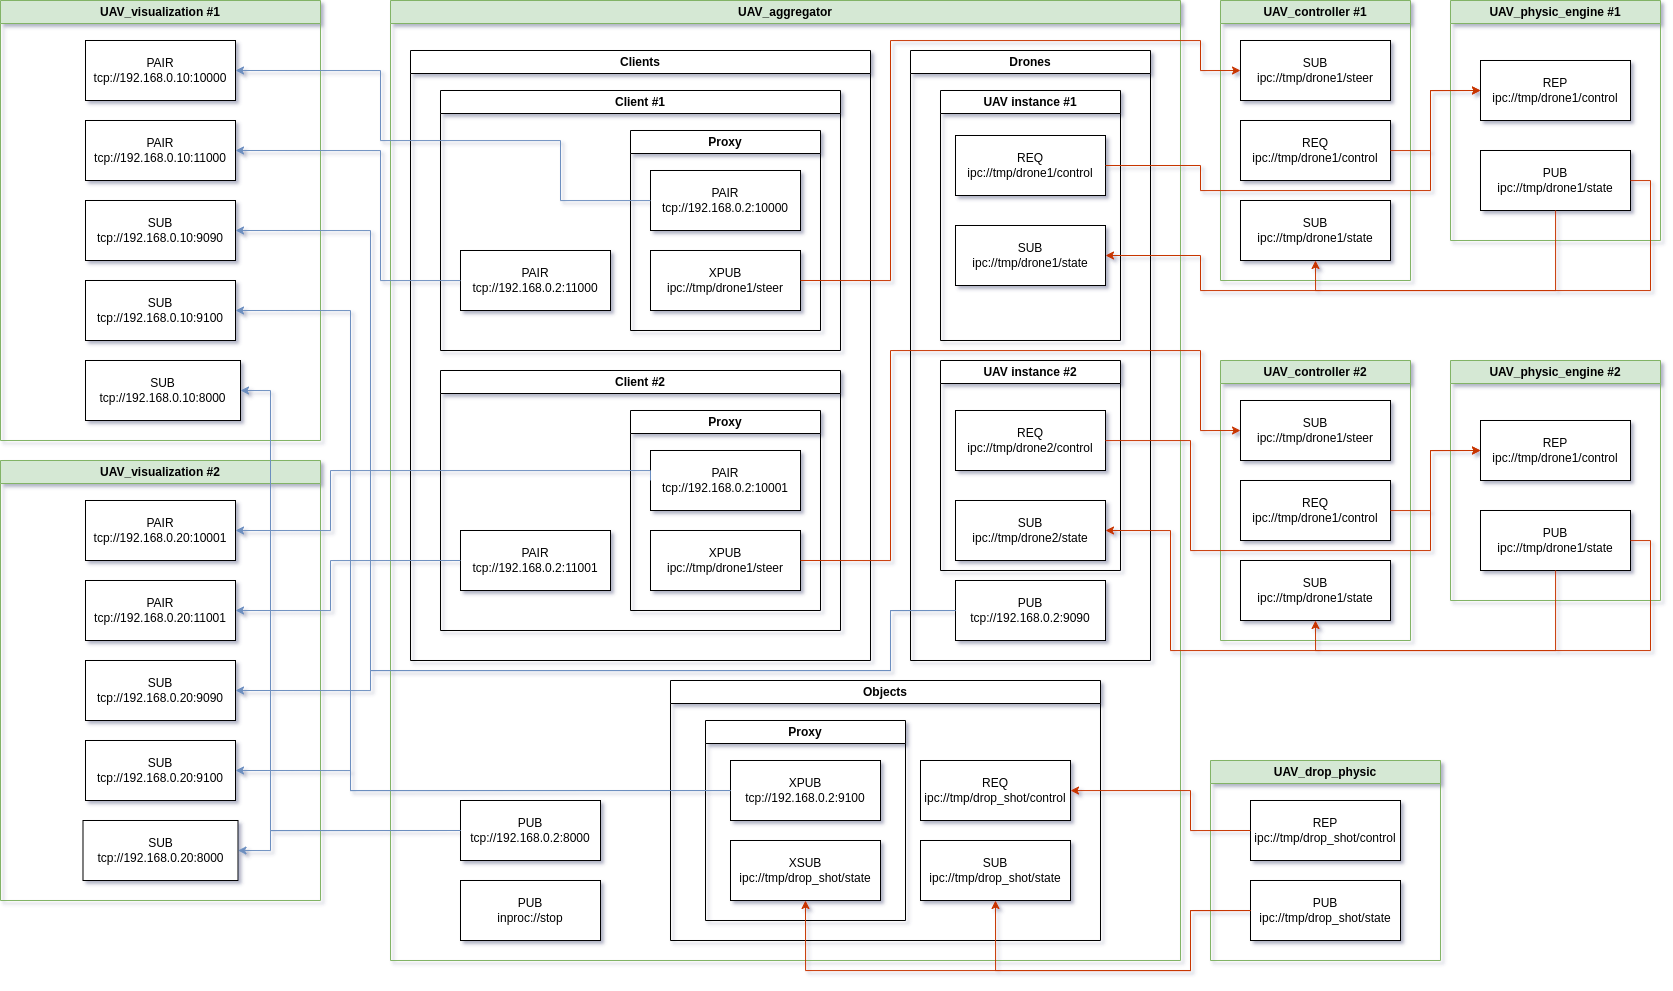
\includegraphics[width=1.2\textwidth, angle=90]{ZMQinMINIUAV.drawio.png}
  \caption{Schemat komunikacji}
  \label{comm}
 \end{figure}

\newpage

\section{Graficzny interfejs użytkownika}

Graficzny interfejs użytkownika składa się z interfejsu serwera oraz interfejsu wizualizacji. 

\subsubsection*{Serwer}

Interfejs serwera zawiera komunikaty dotyczące pracy agregatora oraz otrzymywane od poszczególnych modułów, które są wyświetlane w oknie konsoli. Komunikaty są dodatkowo oznaczone różniącymi się kolorami dla poszczególnych modułów, jak pokazano na rysunkach (\ref{gui_server1}), (\ref{gui_server2}) i (\ref{gui_server3}).

\subsubsection*{Wizualizacja}

Interfejs graficzny wizualizacji składa się z okna konfiguracji przypisań kontrolera pokazanego na rysunku (\ref{gui_bindings1}), ekranu ładowania widocznego na rysunku (\ref{gui_loading}) oraz właściwego widoku wizualizacji ukazanego na rysunkach (\ref{gui_game1}), (\ref{gui_game2}), (\ref{gui_game3}) i (\ref{gui_game4}). \\

Graficzny interfejs użytkownika w wizualizacji składa się z widoku jednej z kamer do wyboru oraz kokpitu. Kokpit w lewym dolnym rogu zawiera radar pozwalający na wykrycie BSP w okolicy. W prawym dolnym rogu znajduje się schemat silników BSP, gdzie możemy odczytać ich prędkości obrotowe. W prawym górnym rogu jest pokazany stan wyposażenia kontrolowanego BSP. Ponadto na kokpicie na dole ekranu znajduje się sztuczny horyzont, którego wizualizacja zgodna jest z powszechnie stosowaną konstrukcją. Pozwala on na uzyskanie informacji o pozycji BSP w przestrzeni, jego orientacji i prędkościach. W lewym górnym rogu sztucznego horyzontu znajduje się obecny tryb lotu BSP. Użytkownik może również włączyć tryb mapy, aby zobaczyć swoje położenia w świecie symulacji.

\newpage
\begin{figure}[!h]
	\centering
	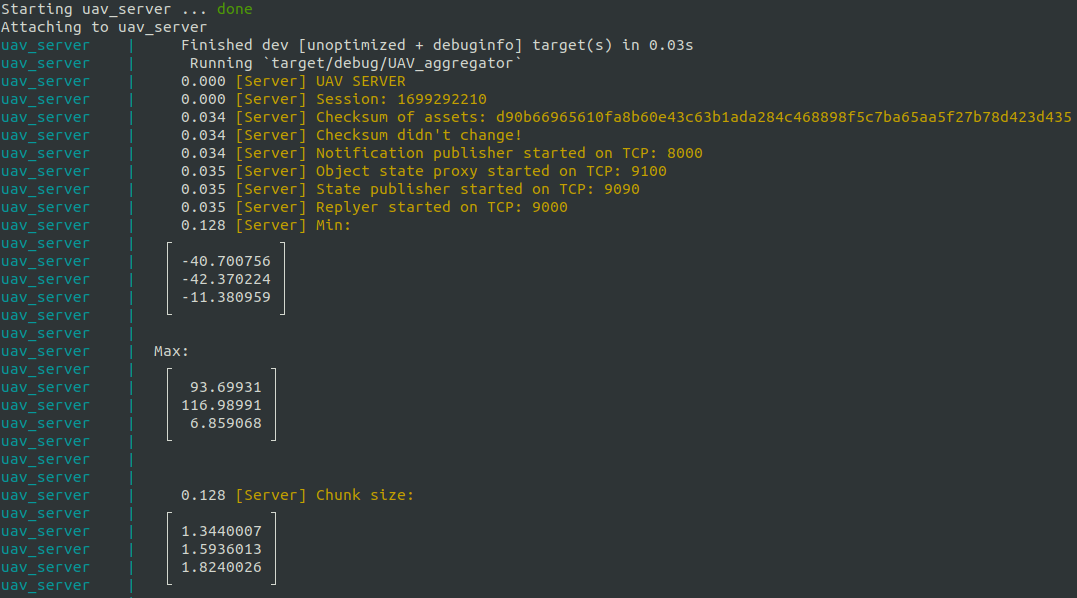
\includegraphics[width=1\textwidth]{gui_server_start.png}
	\caption{Interfejs graficzny serwera w momencie startu.}
	\label{gui_server1}
\end{figure}

\begin{figure}[!h]
	\centering
	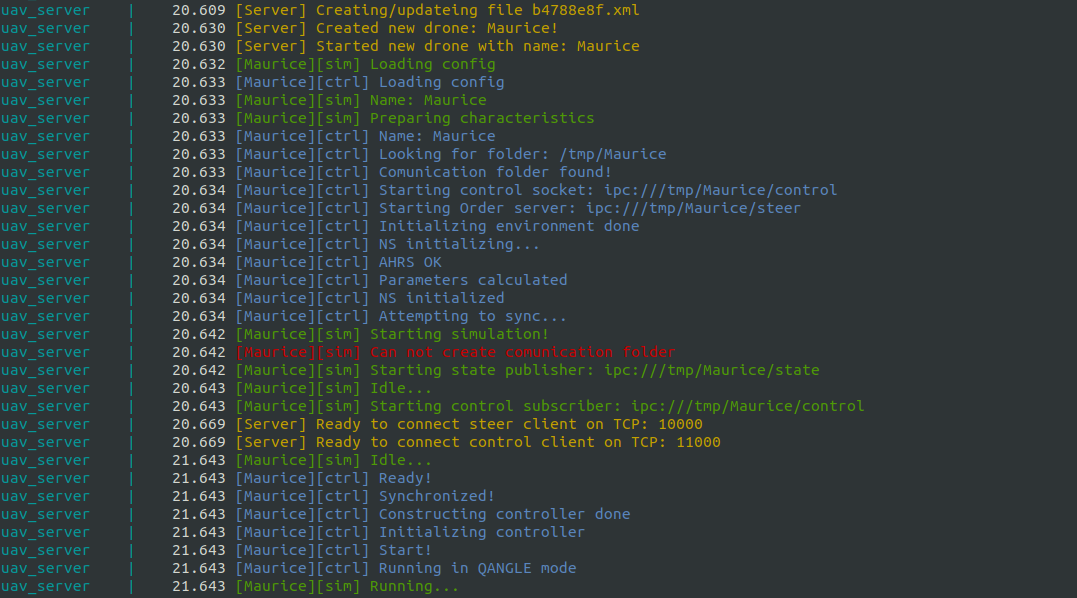
\includegraphics[width=1\textwidth]{gui_server_drone.png}
	\caption{Interfejs graficzny serwera w momencie dołączenia nowego klienta wizualizacji.}
	\label{gui_server2}
\end{figure}

\begin{figure}[!h]
	\centering
	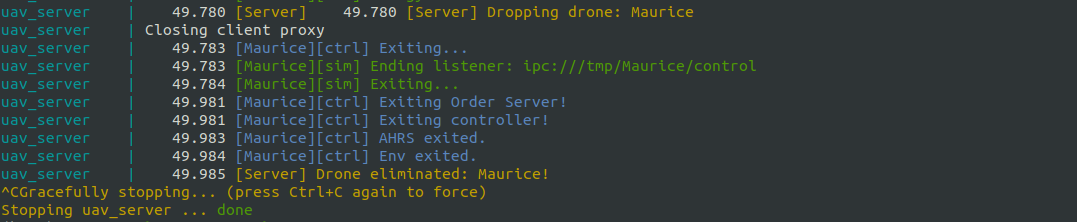
\includegraphics[width=1\textwidth]{gui_server_exit.png}
	\caption{Interfejs graficzny serwera w momencie wyłączenia serwera.}
	\label{gui_server3}
\end{figure}
\begin{figure}[!h]
	\centering
	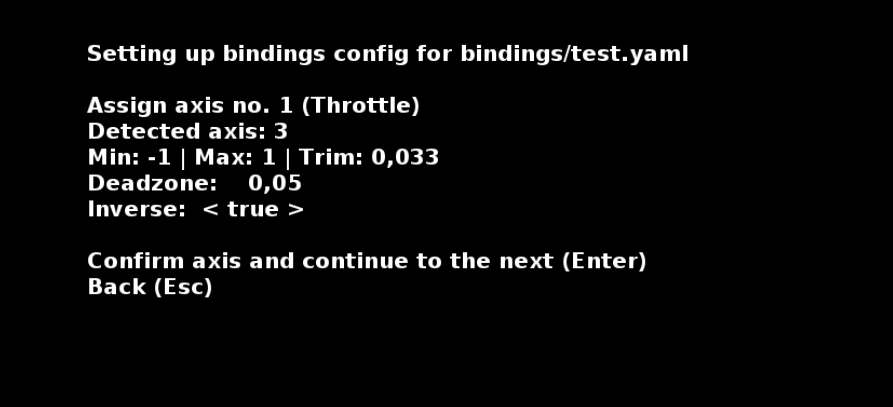
\includegraphics[width=1\textwidth]{bindings1.png}
	\caption{Ekran przypisania osi sterowania.}
	\label{gui_bindings1}
\end{figure}

\begin{figure}[!h]
	\centering
	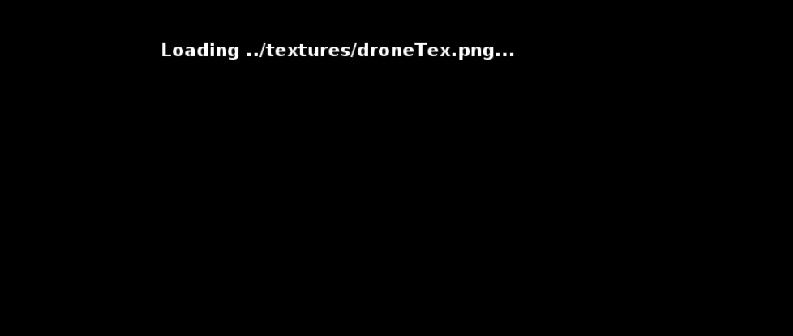
\includegraphics[width=1\textwidth]{loading_screen.png}
	\caption{Ekran ładowania.}
	\label{gui_loading}
\end{figure}

\newpage
\begin{figure}[!h]
	\centering
	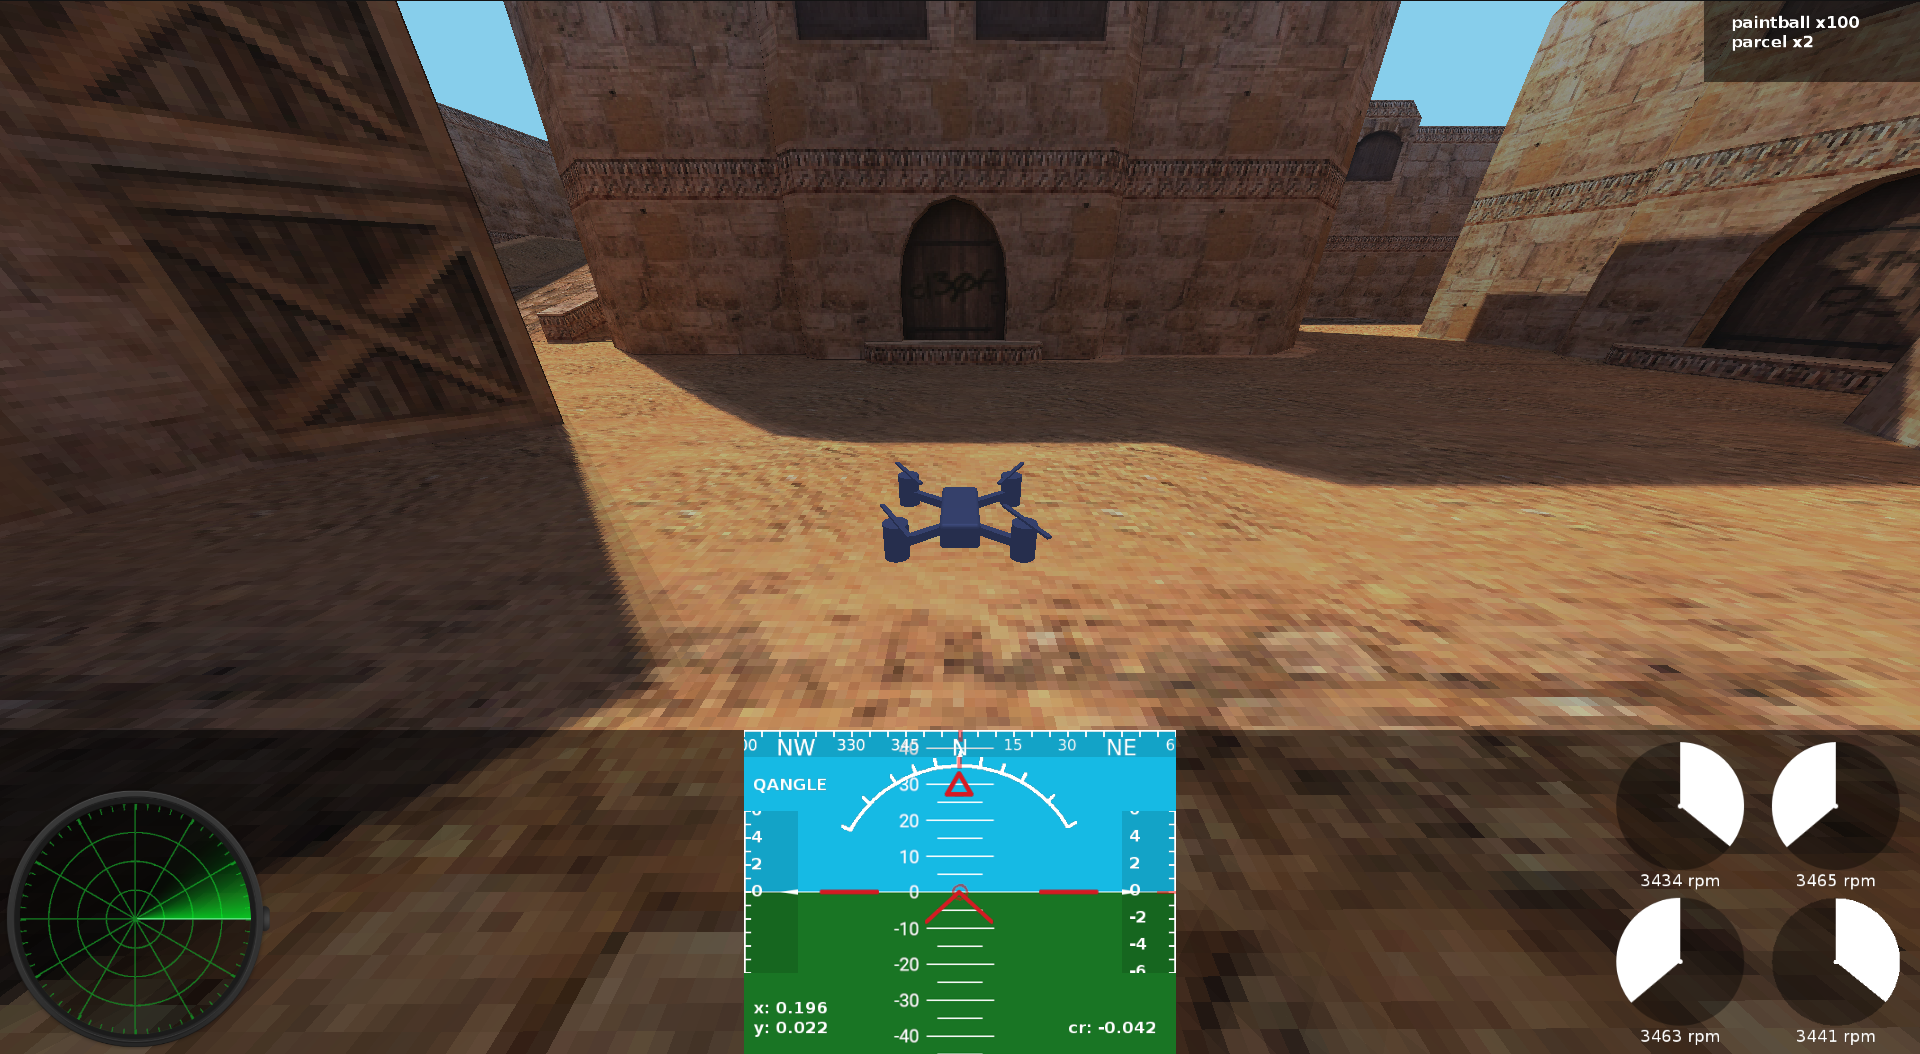
\includegraphics[width=1\textwidth]{game_view.png}
	\caption{Interfejs graficzny wizualizacji w widoku trzecioosobowym.}
	\label{gui_game1}
\end{figure}

\begin{figure}[!h]
	\centering
	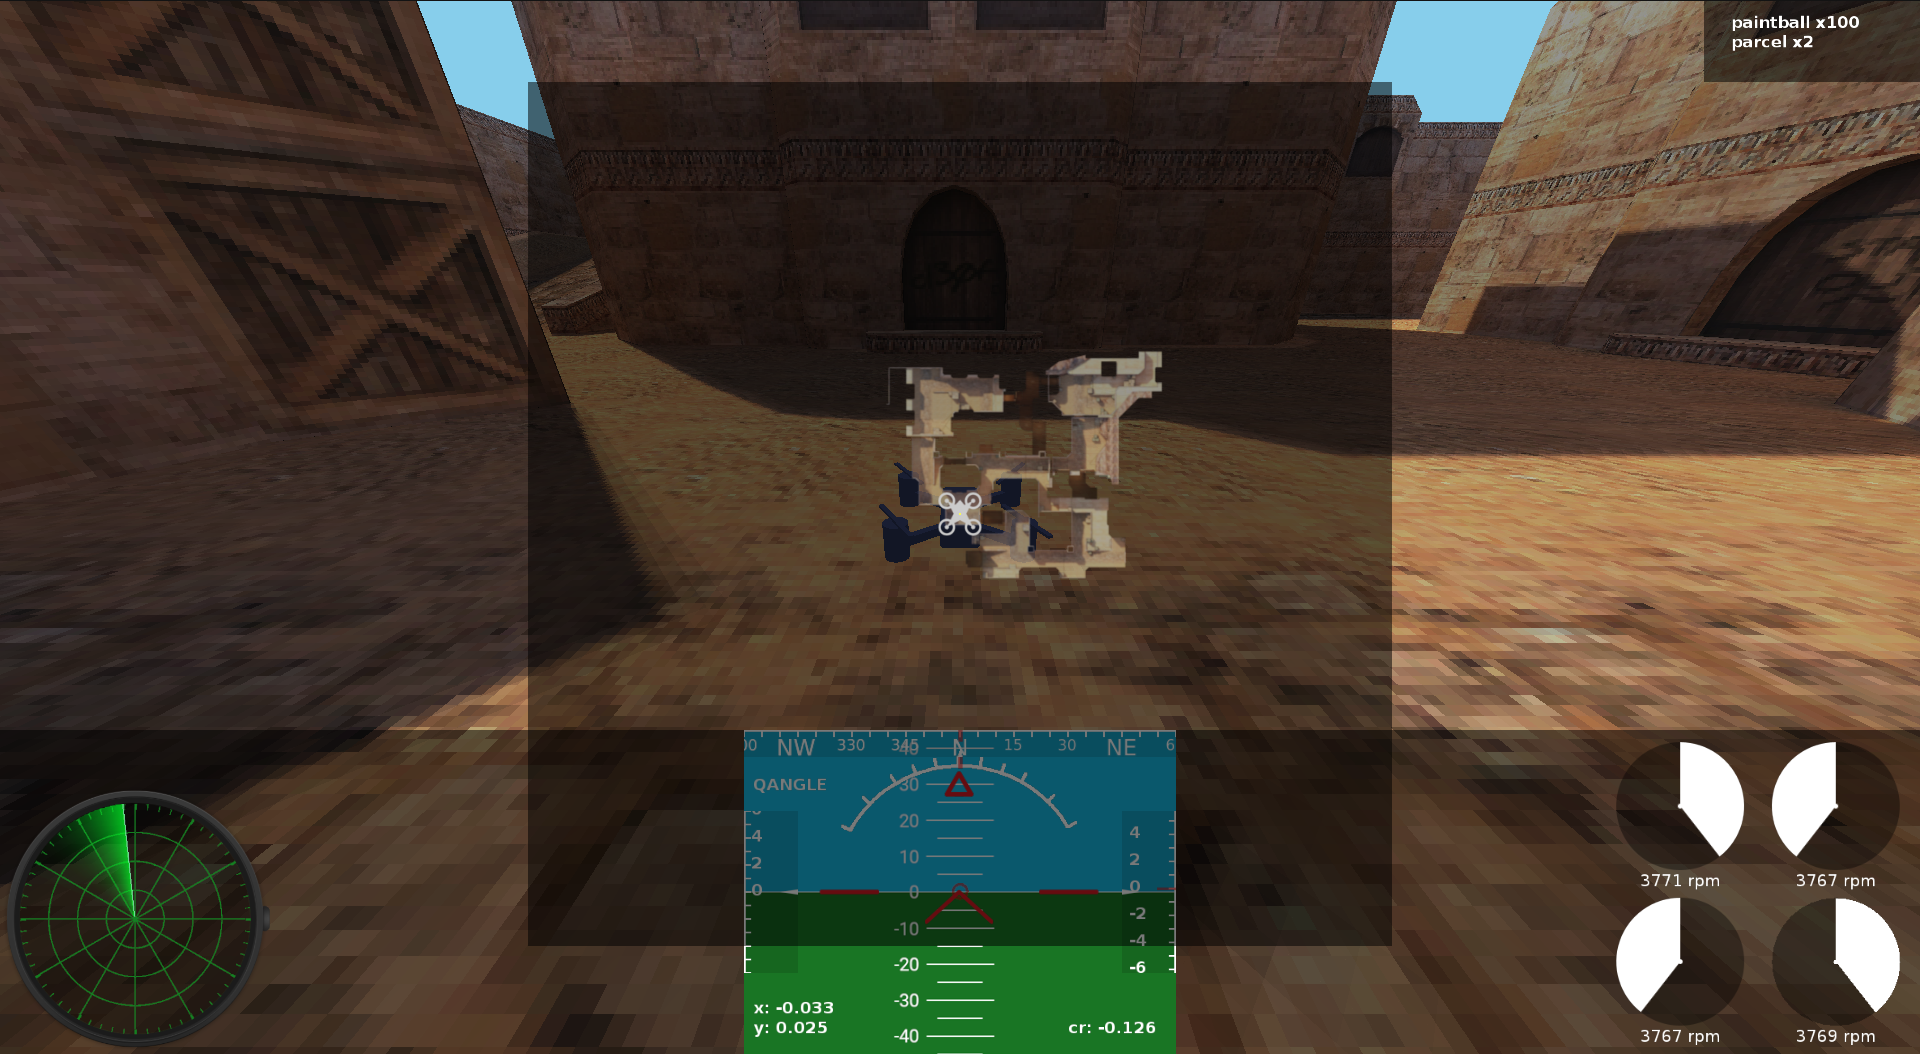
\includegraphics[width=1\textwidth]{game_view_map.png}
	\caption{Interfejs graficzny wizualizacji z włączonym widokiem mapy.}
	\label{gui_game2}
\end{figure}

\newpage
\begin{figure}[!h]
	\centering
	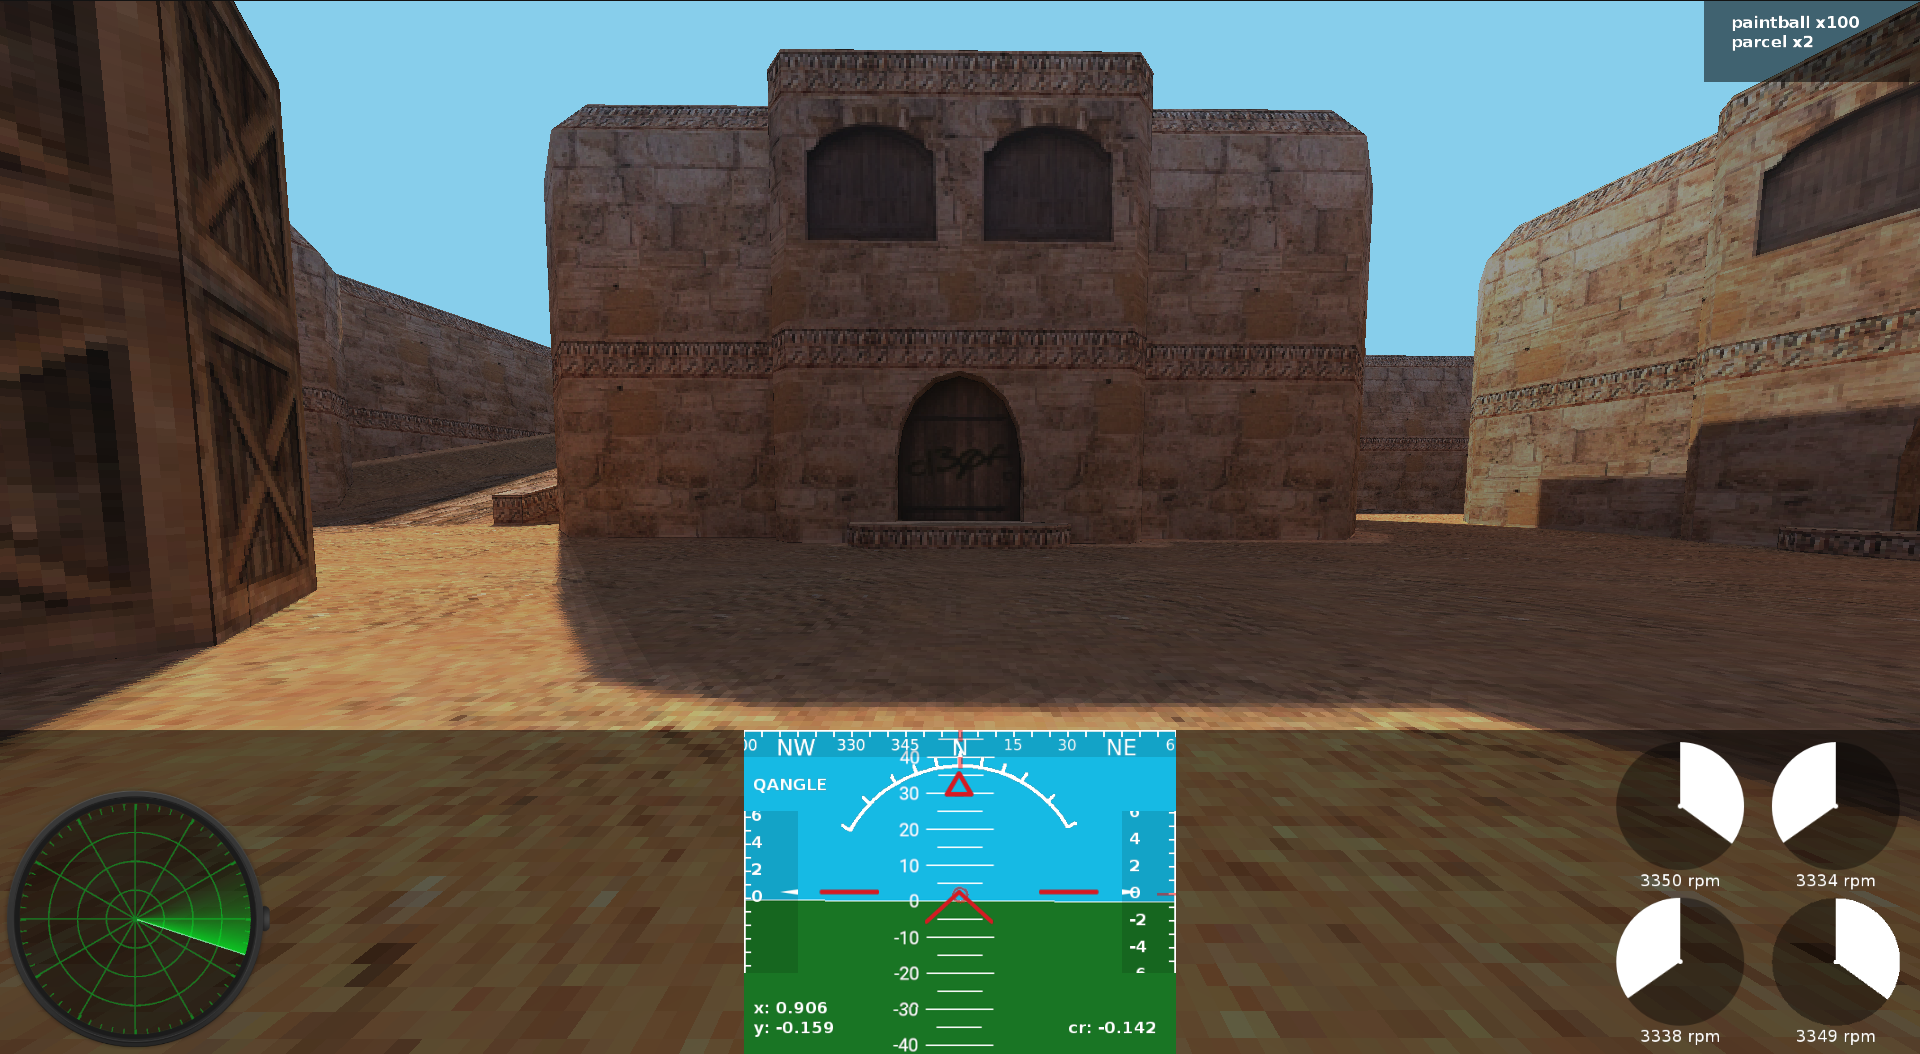
\includegraphics[width=1\textwidth]{game_view_fpp.png}
	\caption{Interfejs graficzny wizualizacji w widoku pierwszoosobowym.}
	\label{gui_game3}
\end{figure}

\begin{figure}[!h]
	\centering
	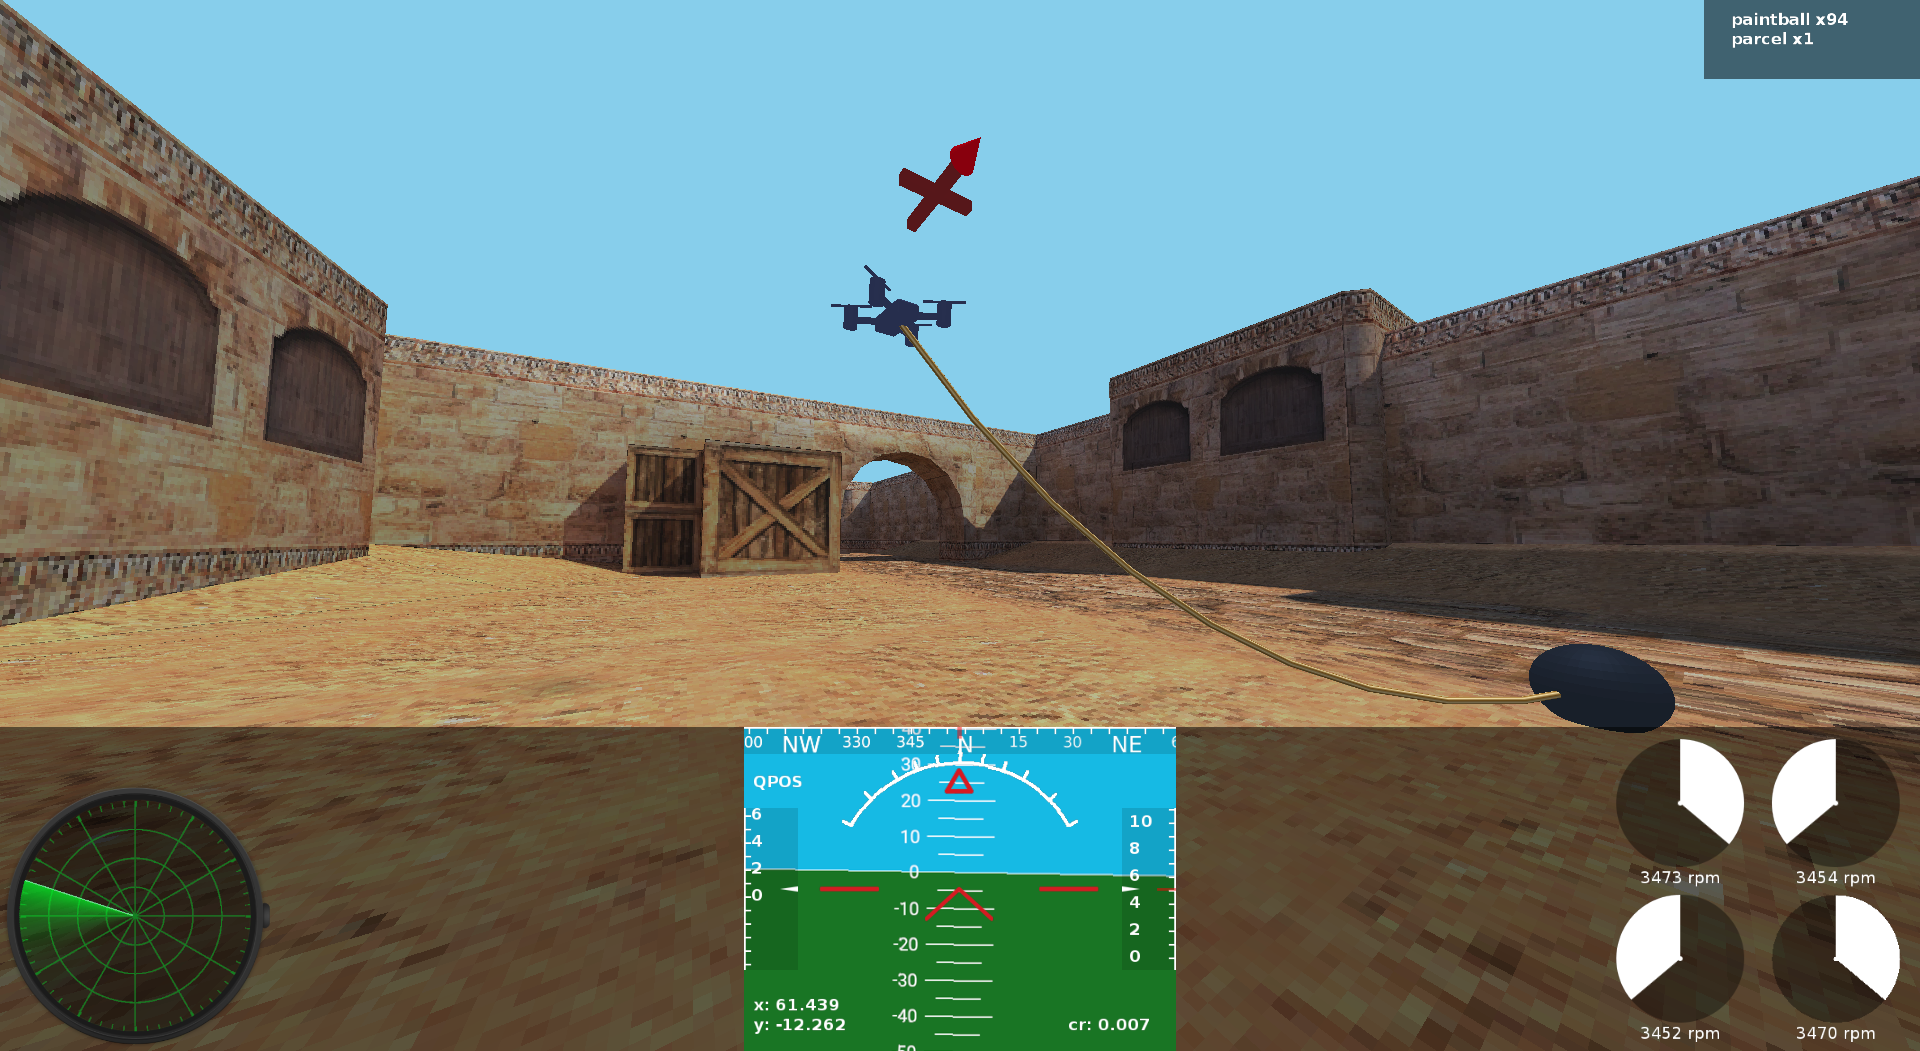
\includegraphics[width=1\textwidth]{game_view_rope.png}
	\caption{Interfejs graficzny wizualizacji w widoku obserwatora i pozycyjnym trybie lotu z opuszczonym ładunkiem na linie.}
	\label{gui_game4}
\end{figure}

\newpage
\section{Interfejs zewnętrzny}

Konfiguracja systemu przed uruchomieniem odbywa się poprzez modyfikację plików konfiguracyjnych i zasobów (asset'ów). Pliki konfiguracyjne dotyczą:

\begin{itemize}
\item Parametrów symulowanego statku powietrznego --\\ UAV\_aggregator/configs/template.xml
\item Parametrów agregatora -- UAV\_aggregator/configs/config.yaml
\item Parametrów wizualizacji -- UAV\_visualization/config.yaml
\item Parametrów kontrolera --  UAV\_visualization/bindings/template.yaml
\item Opisu dostępnych trybów lotu --\\ UAV\_aggregator/assets/data/available\_control\_modes.yaml
\end{itemize}

Pliki konfiguracyjne zostały w całości skomentowane przy pomocy komentarzy odpowiednich dla plików XML oraz YAML  i załączone do pracy.\\


Zasoby zawierają modele i grafiki niezbędne do pracy wizualizacji. Wersja zasobów to pierwsze 8 znaków sumy kontrolnej, która jest generowana na podstawie zawartości assetów i przekazywana wizualizacji przez serwer. Pozwala to użytkownikowi pobrać brakujące zasoby w razie, gdy ich jeszcze nie posiada. Pobrana zawartość jest umieszczana w katalogu od nazwie będącej wersją zasobu. Zasób zawiera następujące katalogi:

\begin{itemize}

\item \textbf{Drones} -- folder zawierający modele 3D statków powietrznych. Zawiera foldery odpowiadające poszczególnym BSP. Nazwa folderu jest tożsama z nazwą BSP.
\begin{itemize}
\item \textbf{\textbf{\textit{NazwaModeluBSP}}} -- Katalog zawierający modele wraz z teksturami dla konkretnego modelu BSP w folderach \textbf{model} i \textbf{textures}.
\end{itemize}

\item \textbf{Maps} -- folder zawierający modele 3D map, które mogą zostać wykorzystane w symulacji. Zawiera foldery odpowiadające poszczególnym mapą. Nazwa folderu jest tożsama z nazwą mapy.
\begin{itemize}
	\item \textbf{\textbf{\textit{NazwaMapy}}} -- Katalog modeli danej mapy. Zawiera modele oraz tekstury mapy w folderach \textbf{model} i \textbf{textures}. W folderze \textbf{model} dodatkowo znajduje się obraz mapy z lotu ptaka pod nazwą "minimap.png".
\end{itemize}

\item \textbf{Data} -- folder zawierający wspólne pliki konfiguracyjne. Obecnie zawiera następujące pliki:
\begin{itemize}
	\item "available\_control\_modes.yaml" -- Plik konfiguracyjny zawierający dozwolone tryby kontroli lotu.
\end{itemize}

\item \textbf{Core} -- folder zawierający pozostałe modele 3D i elementy interfejsu. Zawiera następujące podfoldery:
\begin{itemize}
	\item \textbf{GUI} -- Grafiki niezbędne do wyświetlenia elementów interfejsu graficznego użytkownika.
	\item \textbf{projectile} -- Model i tekstury pocisku w katalogach \textbf{model} i \textbf{textures}.
	\item \textbf{xMark} -- Model i tekstury markera 3D w katalogach \textbf{model} i \textbf{textures}.
\end{itemize}

\end{itemize}

W katalogach \textbf{model} zawarty jest model obiektu w postaci pliku z rozszerzeniem GLTF, a więc "model.gltf" wraz z odpowiadającym mu "model.bin" oraz pliku z rozszerzeniem OBJ: "model.obj". Plik GLTF wykorzystywany jest w wizualizacji, a OBJ służy rozpoznawaniu kolizji.\\


W zasobie znajduje się również tekstura domyślna ładowana w przypadku nieznalezienia wymaganej tekstury.\\


\newpage


\section{Dobór technologii} \label{technologies}

Do realizacji poszczególnych modułów wybrane zostały następujące narzędzia programistyczne i biblioteki zewnętrzne.\\

\noindent\textbf{UAV\_physic\_engine, UAV\_controller i UAV\_drop\_physic}\\
Ze względu na duży nakład obliczeniowy -- symulacja w czasie rzeczywistym z krokiem całkowania rzędu 1ms -- wybrany został język C++. Z uwagi na swoją wydajność i elastyczność stanowi on naturalny wybór w wydajnych symulacjach komputerowych. Dodatkowo wykorzystane zostały następujące biblioteki:
\begin{itemize}[noitemsep,nolistsep]
	\item Eigen -- biblioteka zawierająca elementy algebry liniowej: macierze, wektory i~związane z nimi algorytmy. Eigen stawia na wydajność poprzez wykorzystanie rozkładów typu SIMD, przy 		jednoczesnym zachowaniu przejrzystej składni,
	\item ZeroMQ -- binding biblioteki libzmq dla języka C++. Libzmq jest bazową biblioteką implementującą kolejki ZeroMQ w języku C,
	\item RapidXML -- biblioteka do parsowania plików XML,
	\item Cxxopts -- biblioteka do interpretowania argumentów wejściowych programu.
\end{itemize}
\  \\
\textbf{UAV\_aggregator}\\
Do realizacji modułu agregatora wykorzystany zostanie język Rust. Pozwala on na tworzenie wydajnego i kompilowanego kodu przy jednoczesnym zachowaniu przenośności między systemami. Natywnie wspiera zarządzanie innymi procesami i udostępnia wiele bibliotek. Wykorzystane zostały następujące biblioteki:
\begin{itemize}[noitemsep,nolistsep]
	\item nalgebra -- biblioteka zawierająca elementy algebry liniowej, odpowiednik biblioteki Eigen dla języka Rust,
	\item zmq -- binding biblioteki libzmq dla języka Rust.
	\item xmltree -- biblioteka do parsowania plików XML,
	\item merkletree -- biblioteka wykorzystana do hashowania drzewa plików,
	\item sha1 -- biblioteka wykorzystana do hashowania plików konfiguracyjnych,
	\item serde\_yaml  - biblioteka do parsowania plików YAML.
\end{itemize}
\  \\
\textbf{UAV\_server}\\
Do realizacja kontenera wybrane zostało oprogramowanie Docker. Obraz został zdefiniowany przy pomocy Dockerfile i skryptów Bash. Przygotowany został również plik Docker compose ułatwiający uruchomienie serwera.\\
\noindent\textbf{UAV\_visualization}\\
Do zrealizowania wizualizacji zostanie wykorzystany język Java. Obiektowość języka pozwoli na wytworzenie przejrzystej implementacji łatwej w utrzymaniu. Zaletą tego wyboru jest również to, że język ten znajduje się na rynku od długiego czasu, dzięki czemu dostępny jest bogaty zasób bibliotek. W opisywanym module zostaną wykorzystane m.in.:
\begin{itemize}[noitemsep,nolistsep]
	\item LWJGL -- Lightweight Java Game Library. Biblioteka udostępniająca bindingi do gamy bibliotek dla deweloperów gier napisanych w języku C, takich jak Vulkan, OpenGL, OpenAL i OpenCL,
	\item JeroMQ -- Natywna implementacja biblioteki libzmq w języku Java.
	\item JOML -- Java OpenGL Math Library. Biblioteka implementująca operacje algebry liniowej przydatne przy implementacji aplikacji renderujących obraz 3D,
	\item Jackson -- Biblioteka do parsowania plików XML i JSON,
	\item Project Lombok -- Biblioteka ułatwiająca pisanie kodu, pozwalając na zastępowanie powtarzalnych fragmentów adnotacjami.
\end{itemize}
\  \\
\textbf{UAV\_map\_generator}\\
Do zrealizowania skryptu automatyzującego został wykorzystany język Python. Skrypt łączy wywołania zewnętrznych programów, niezbędnych do przygotowania mapy na podstawie danych geograficznych pobranych z serwisu OpenSteetMap. W skrypcie zostały wykorzystane m.in.:
\begin{itemize}[noitemsep,nolistsep]
	\item numpy -- moduł zawierający elementy algebry liniowej,
	\item requests -- moduł umożliwiający wykonanie zapytania HTTP,
	\item subprocess -- moduł umożliwiający uruchamianie zewnętrznych programów,
	\item cairosvg -- moduł umożliwiający konwersje plików graficznych,
	\item pygltflib -- moduł służący do modyfikowania plików GLTF,
	\item OSM2World -- program umożliwiające konwersje danych geograficznych do plików zawierających modele 3D,
	\item gltf-pipeline -- moduł NodeJS umożliwiający konwersję plików GLTF.
\end{itemize}

\ \\ 
Każdy z modułów znajduje się w oddzielnym repozytorium Git na platformie Github. Dla ułatwienia pracy z wykorzystaniem Github Actions przygotowane zostały odpowiednie mechanizmy CI/CD.

